\chapter{Introduction}

Life is a beautiful phenomenon. We struggle to find it in other parts of the universe, yet in our planet is everywhere. Even in the most inhospitable places, such as volcanoes and deserts, life flourishes. Also, life comes in different forms as living organisms are roughly classified into five very different kingdoms. Such diversity raises many questions for scientists interested in understanding life. Biophysicists are devoted to revealing the intricacies of living organisms via physics and sometimes chemistry. This novel approach has gained much attention, as physics provides a fundamental vision of the phenomena that allow us to understand them in a broader sense, grouping those with a common interpretation.

Biophysics has addressed topics of various parts of life. There are studies with a physical approach on cell membranes \cite{Nguyen2021PhotocatalyticSynthesis,Jin2020MechanosensitiveMechanisms,Janmey2006BiophysicalMembranes}, biological macromolecules \cite{Allewell2013MolecularSciences, 2008MethodsFunction, Fierz2019BiophysicsDynamics}, evolution \cite{Sikosek2014BiophysicsBiophysics}, bacteria movement \cite{Lauga2020TheMotility, Ananthakrishnan2007TheMovement}, diseases such as cancer and Alzheimer's \cite{White2019TheCancer, Weickenmeier2019ASclerosis} and much else. Physics has already brought to these topics fundamental explanations, which contributed to typically descriptive biology in the quest to understand life. Biophysics has proven its usefulness in a few decades.

This thesis focuses on studying the interaction between bacteria and sinusoidal walls from a biophysical point of view to control or reduce biofilm formation.

\section{Biofilm}

Biofilms are consortiums of cells living on a surface. These cells secrete polymers, typically proteins and polysaccharides, which form an extracellular matrix that the cells share. Mechanisms employed in biofilm formation vary depending on strains and environmental conditions. Biofilm is a structure challenging to deal with, as antibiotics have proven to fail at killing bacteria in biofilm even at a concentration 1000 times higher than the normal concentration that kills floating bacteria \cite{Costerton1987BacterialDisease.}. This means that biofilm is a chronic bacterial infection.

\afterpage{%
\begin{figure}[H]
	\centering
	\includegraphics[width=\linewidth]{imagenes/BiofilmFormation.PNG}
	\caption[Diagram of biofilm formation]{ Diagram of biofilm formation in chronological order. a) Reversible association of a bacteria with a surface. b) Irreversible adhesion of bacteria, due to chemical or physical reasons. c) Cellular division leads to formation of microcolonies and aftwerwards d) biofilm structure is complete. (from \cite{Costerton1987BacterialDisease.})}
	\label{biofilm}
\end{figure}
}

Biofilm was not a problem in the early development of health care because it is relatively rare to have this kind of infection inside the human body. Due to this, biofilm was the last of the problems, but this has changed recently. This change relies on the cause of biofilm formation in the human body. ``The inability of the host and of therapeutic efforts to resolve acute infection triggers a series of events that culminates in a chronic condition" \cite{CiernyIII2006TreatmentInfection}. Diabetes and intra-corporal devices are contemporary reasons that decrease the ability of the body to resolve an infection, so biofilm appears. Badly treated diabetes can produce chronic hyperglycemia, associated with failure of blood vessels among many other organs \cite{2014DiagnosisMellitus}. This reduces wound healing as less blood reaches the wound; therefore, people with diabetes are an at-risk group for biofilm formation.

On the other hand, intra-corporal devices are made to replace something on a human body, compensating for the missing function. The problem is that intra-corporal devices are like dead tissue for the immune system. This means that any bacteria that attach to this surface will be harder to reach. These device-related infections have interrupted the development of complex medical devices that could replace organs like the heart. If these mechanical organs are susceptible to infections, they bring more problems than solutions \cite{Costerton1999IntroductionBiofilm}. Considering this, developing technology that prevents biofilm formation has brought interest as it could allow new medical technology.

\subsection{Objective: interrupt biofilm formation}

Biofilm formation begins with the association of a bacterium to a surface. This means that the bacteria are near or in contact with the surface. Bacteria are attracted to the surface due to hydrodynamic effects, and some species can even sense the presence of a surface by signaling molecules. This state of association is reversible as bacteria are still moving on the surface. Depending on the species, bacteria may move very little or explore the surface before adhering \cite{Costerton1999IntroductionBiofilm}. Once adhered, due to chemical or physical reasons, the process is irreversible. The cell will divide, forming microcolonies of bacteria whose secretions will form the extracellular matrix that composes the biofilm. Therefore, to reduce biofilm formation, it is essential to revert the association of bacteria with a surface before the adhesion takes place. To do so, the chemical and physical properties of the surface must be tweaked.

Considering the above, the objective of this thesis is to \textbf{generate a surface that makes bacteria move away from it due to its sinusoidal geometry}, thus preventing cell adhesion. This will be done experimentally in in vitro systems, i.e., in controlled non-living environments. In addition, \textbf{a model of the system will be generated to pursue a fundamental physical explanation of the experimental observations}. This complementation between experiments and simulations will allow a deeper understanding of the results. The rest of the chapter introduces the physical effects that led to this objective. In section \ref{section:active matter} we describe bacteria movement in general and later on focus on \textit{E. coli} the species we used in experiments. Meanwhile, section \ref{section:surface effects} describes the effects of surfaces in bacteria swimming and the idea behind using a sinusoidal surface.

\section{Active matter}
\label{section:active matter}

In this thesis, we focus on the interaction between \textit{E. coli} bacteria and a surface. The area of biophysics that encompasses this subject is known as active matter. Active matter studies complex systems with the perspective that the active motion of every particle is the key to understanding the phenomena. Active motion refers to the idea that a particle obtains energy from the medium to propel itself. This is a common feature of organisms such as prokaryotic cells and animals. Interactions between particles or their environment lead to fascinating phenomena. Flock of birds \cite{Bialek2012StatisticalBirds,Cavagna2015FlockingMotion}, schools of fish \cite{Toner1998FlocksFlocking}, bacterial suspensions \cite{Lopez2015TurningSuperfluids, Clement2016BacterialFlow,Vincenti2019MagnetotacticMotor}, crowds of people \cite{Faria2010LeadershipCrowds} and even artificially active colloidal particles \cite{Zhang2018Light-controlledParticles, Jiang2020PickeringApplications} are examples of active matter. Typically, these systems exhibit interesting collective behavior. For example, in flocks and schools, individuals move more or less in the same direction and are able to follow as a whole the change of direction proposed by leaders. This collective movement is a survival method that allows the flock to avoid attack by predators \cite{Bialek2012StatisticalBirds,Cavagna2015FlockingMotion}.


\afterpage{%
\begin{figure}[H]
	\centering
	\includesvg[width=\linewidth]{imagenes/activeMatter}
	\caption[Examples of active matter]{Examples of active matter. Flocks of birds, school of fish and crowds are examples of macroscopical active matter. Bacteria and active colloids on the other hand are microscopical examples. }
	\label{experimental profiles}
\end{figure}
}

\subsection{Bacterial suspensions}

Among these examples, we are interested in the culture of bacteria in fluids, called bacterial suspensions. Bacteria are grown in a rich medium but not necessarily observed in such conditions because by centrifugation, they can be transferred to scarcer media. Bacterial suspensions are put in microscopic environments to study the dynamics of the cells. This is attractive because the behavior of bacteria can be controlled by using different species or even by genetic modifications. Individuals of the same species \textit{E. coli} can move in straight lines instead of doing tumbles just by changing one gene \cite{VanVliet2014ThePopulations}. Genetic modifications produce new species strains that can better suit a specific study. Such possibilities make bacterial suspensions the playground of choice for active matter studies.

Bacteria have different mechanisms to move depending on their natural habitat. In solid surfaces, bacteria move through twitching, gliding, or usage of flagella. Flagella-driven movement is the most common type of movement, and it also allows swimming in liquids. Flagella structure has three parts, the basal body that produces rotation, the filament, a helical propeller, and the hook that connects both structures transmitting the torque from the body to the filament \cite{Nakamura2019Flagella-drivenBacteria}. Different species may have differently composed flagella and also a different number of flagella (see figure \ref{flagella}). 


\afterpage{%
\begin{figure}[H]
	\centering
	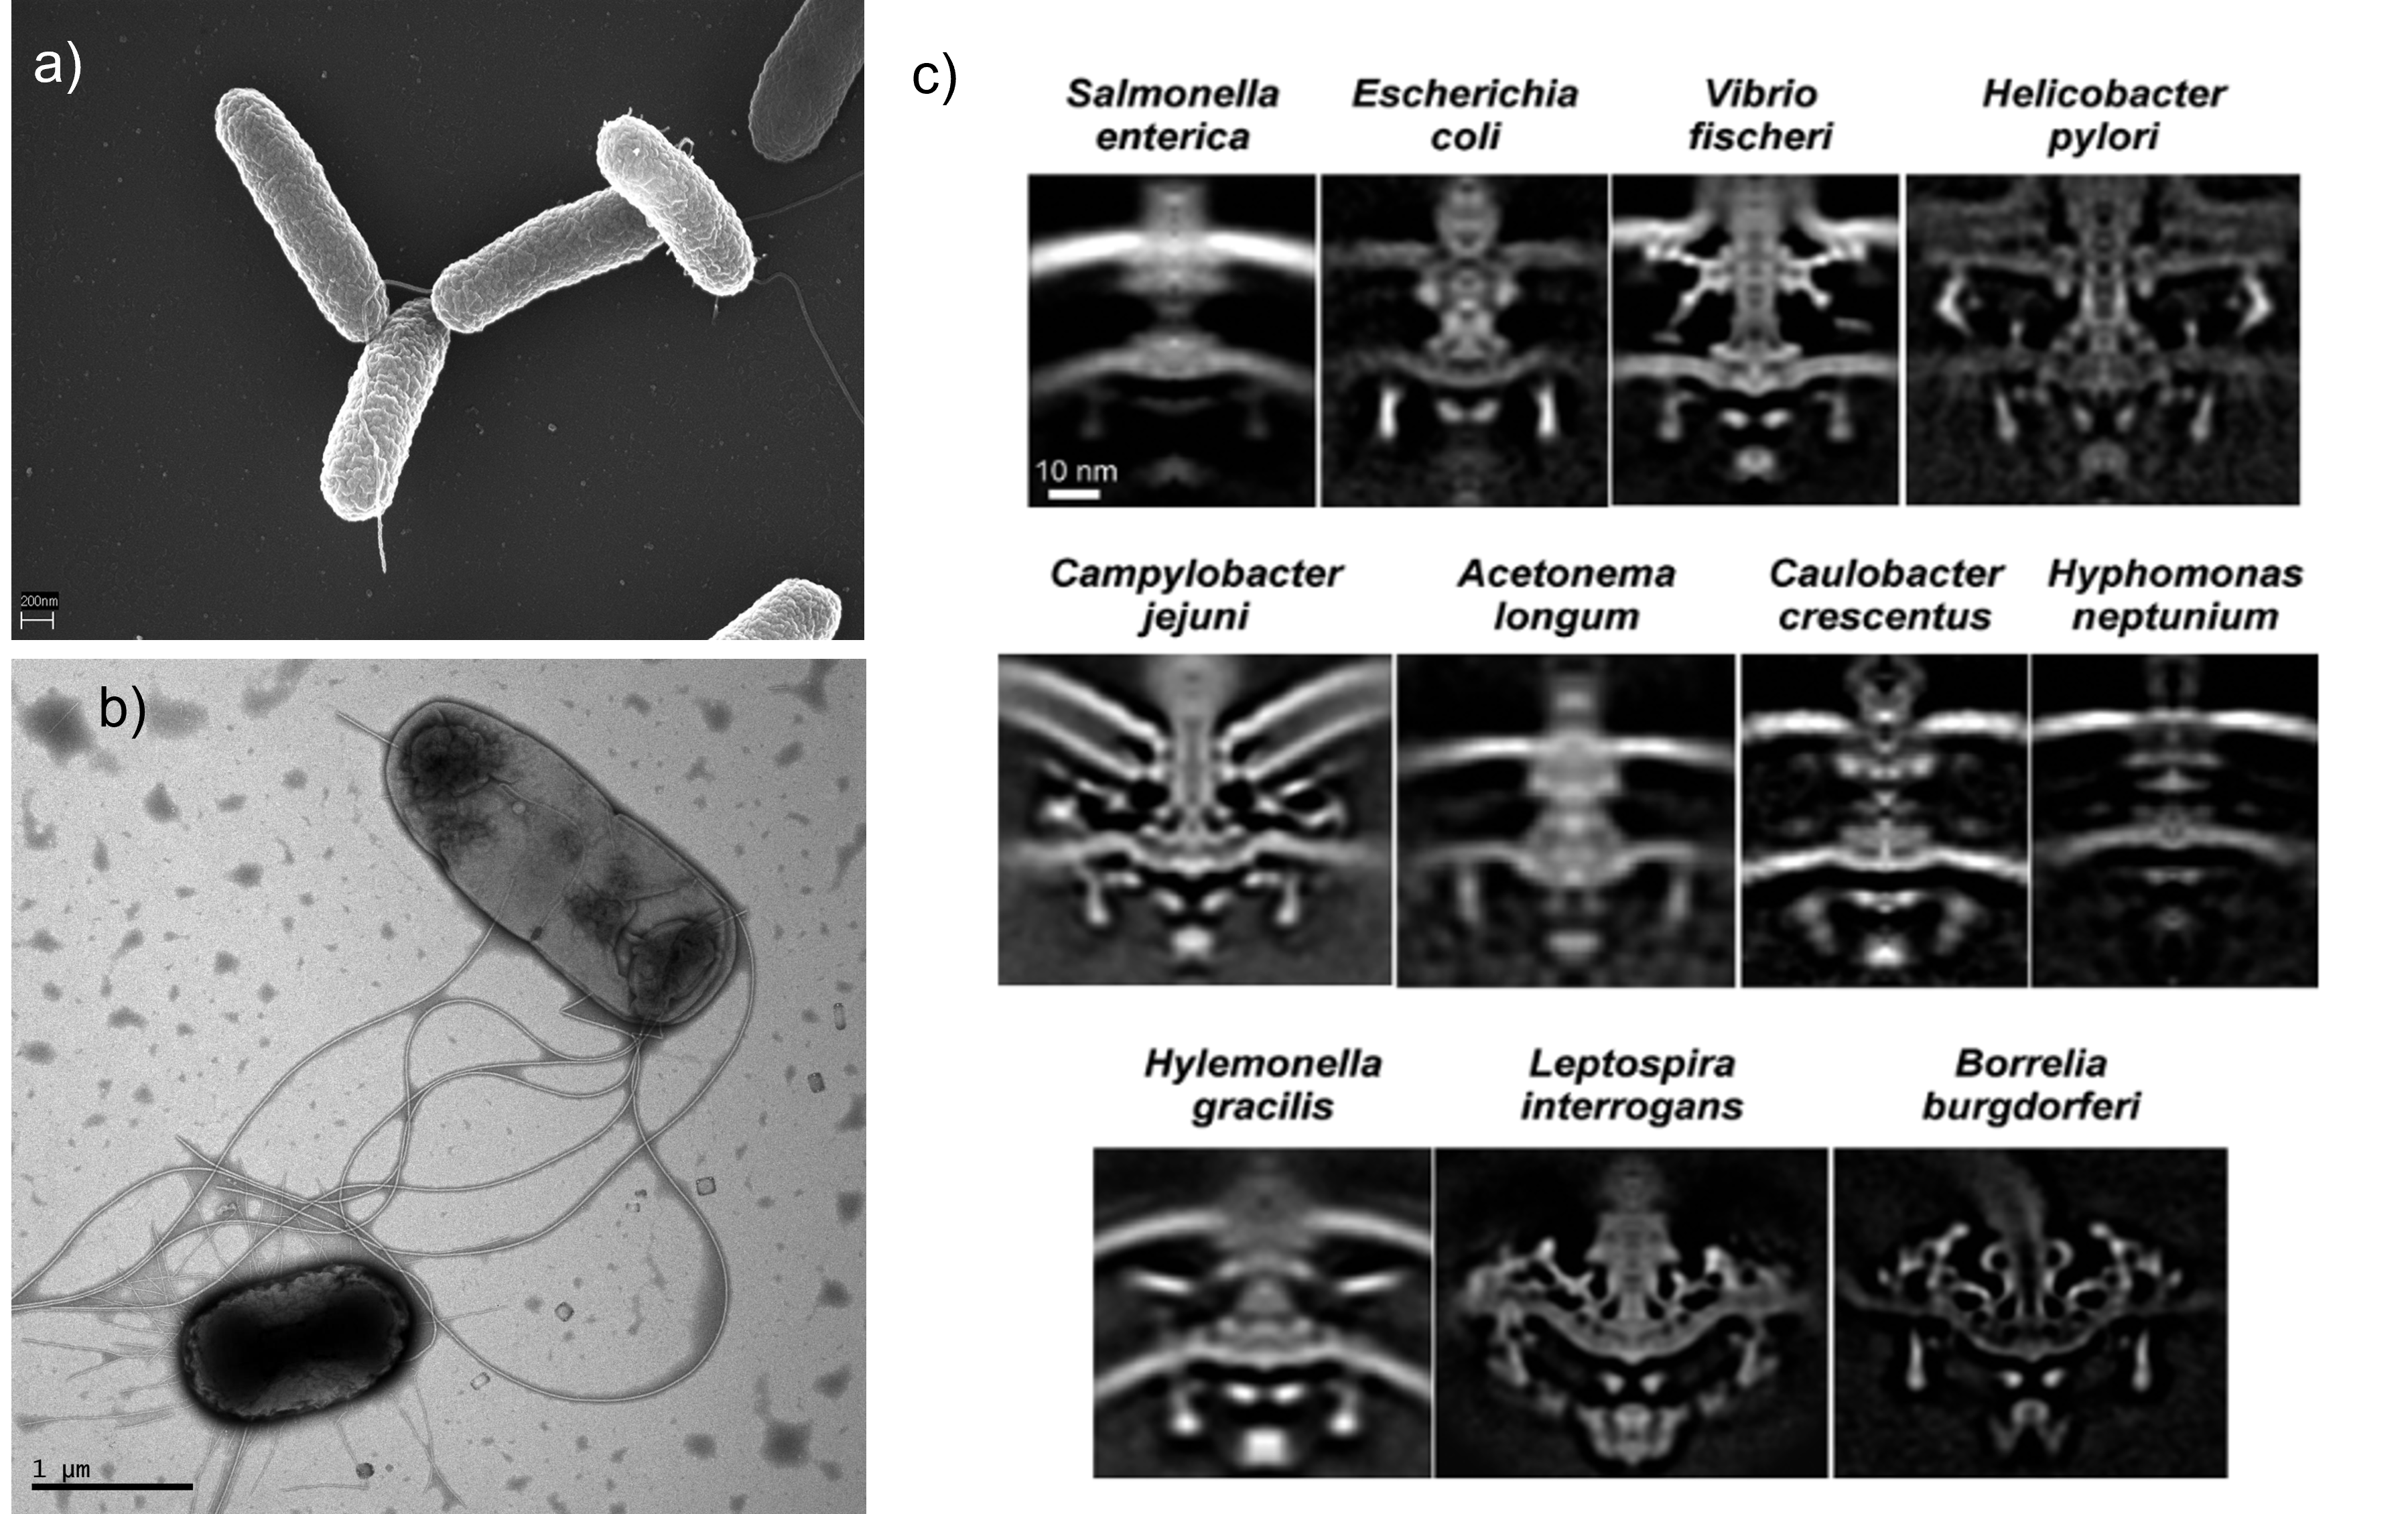
\includegraphics[width=\linewidth]{imagenes/flagella_full.png}
	\caption[Comparison of bacteria flagella of different species]{Electron micrographs of a) \textit{Salmonella} and b) \textit{E. coli} cells. Position and number of flagella are different. c) Structural differences in the basal body among bacterial species observed with electron cryotomography.  (adapted from \cite{Nakamura2019Flagella-drivenBacteria, Terashima2017StructuralSpecies}).  }
	\label{flagella}
\end{figure}
}



When swimming, the flagella of bacteria move coordinately to propel the body in one direction. This movement propels the bacteria with a force $\textbf{F}$. The body of the bacteria also experiments a drag force $-\textbf{F}$ due to the fluid resistance. Therefore, the effect of bacteria movement in fluids is modeled as a force dipole. This description has one degree of freedom called polarity. Polarity reveals whether the bacteria push or pull the fluid. Pushers have their flagella at the rear while the pullers have them at the front. An alternative description is that the pushers produce a flow away from their bodies, while pullers produce the opposite. In figure \ref{swimming methods} d) it is possible to see a comparison between the flow produced by these two swimming mechanisms. Flow-induced by bacteria produce hydrodynamic interactions between cells and also with surfaces. Such interactions have been extensively studied, and the effects of interest to us will be discussed in the following section. 

\afterpage{%
\begin{figure}[H]
	\centering
	\includesvg[width=\linewidth]{imagenes/swimming_methods}
	\caption[Force dipole approximation for bacteria swimming effects in fluids.]{a) Experimentally measured average flow flied produced by single \textit{E. coli}. b) Best-fit force dipole flow and c) the subtraction of the best-fit flow and the measured field. Parameters for the fitting include the magnitude of the forces $|\textbf{F}| =$ \SI{0.42}{\pico\newton} and the separation $\mathscr{l} =$ \SI{1.9}{\micro\meter} between the two forces (taken from \cite{Drescher2011FluidScattering}). d) Comparison between flows produced by spherical pushers and pullers in numerical simulations when moving upwards (taken from \cite{Zhu2012Self-propulsionPullers}).}
	\label{swimming methods}
\end{figure}
}

\subsection{\textit{Escherichia coli}}

In our study, we use the species of bacteria \textit{E. coli} because it is the most studied bacterial species. For example, as seen in figure \ref{swimming methods}, it has been proven that the first-order approximation of the dipole force scheme fits properly the flow produced by  \textit{E. coli} swimming at long ranges\cite{Drescher2011FluidScattering}. Near-field effects are not captured accordingly. Also, physical properties of \textit{E. coli} have been measured. Cells are rod-shaped and are about \SI{2}{\micro\meter} long and \SIrange[range-units=single]{0.5}{1}{\micro\meter} in diameter \cite{BritannicaOnlineEncyclopedia2021EducationEncyclopedia}. \textit{E. coli} produces around $5$ to $10$ flagella randomly distributed across the cell surface. When moving in straight lines or in a ``run", these flagella form a bundle that rotates in a counter-clockwise direction (when seen from behind). If any flagella start rotating clockwise, the bundle disassembles, and bacteria changes the direction of motion or ``tumbles". This movement is described as a run-and-tumble motion. The basal body of \textit{E. coli} rotates at \SI{10}{\hertz} and the typical tumble duration is \SI{0.1}{\second} \cite{Berg2001E.ColiMotion}. We measured the average speed of an \textit{E. coli} culture to be around \SIrange[range-units=single, per-mode = symbol]{18}{25}{\micro\meter \per \second}. The average speed depends on culture conditions such as temperature, oxygen presence, and manipulation. 

The specie \textit{E. coli} also has many mutant variations. It has been proven that up to $80\%$ of the genes in a typical genome of \textit{E. coli} are variable or ``accessory" genes \cite{Lukjancenko2010ComparisonGenomes}. In laboratories, \textit{E. coli} strains normally have a gene for expressing green (GFP) or red (mCherry) fluorescent proteins, allowing observation of bacteria only. For active matter studies, in particular, the most common genetic modification corresponds to the elimination of the synthesis of the cheY protein. This protein is involved in the transmission of sensory signals from the chemoreceptors to the flagellar motors, or in other words, regulates the chemotaxis in the cell. Therefore, cheY deletion causes the cell to stop tumbling. This is useful for studying particular properties of the swim that are independent of the tumbles or to avoid effects produced by tumbling and. We use this type of genetic modification in our experiments. Another typical example of genetic modifications is \textit{E. coli} strains rendered non-motile via deletion of motility proteins and then restored motility via inducible expression of the deleted gene from a plasmid. Other bacteria or a specific signal can regulate the induction. These strains lead to interesting dynamics, such as pattern formation and directed movement \cite{Ravichandar2017TranscriptionalGradient, Curatolo2020CooperativeRegulation}.

\section{Surface effects}
\label{section:surface effects}

\afterpage{%
\begin{figure}[H]
	\centering
	\includegraphics[width=\linewidth]{imagenes/3d_tracking.PNG}
	\caption[Volumetric reconstruction of bacteria during a wall-entrapment event.]{a) A sequence of volumetric reconstructions of swimming cells during a wall-entrapment event. b) A close and lateral view of another cell colliding with the wall. Time intervals between reconstructions are 0.2 s in both figures. (c) For the same cell as in (b), the wall distance is plotted as a black line, while the red line plots the angle of the cell-body axis. In both curves, three stages can be identified: approach to the wall, reorientation, and surface swimming. The grey shaded areas help to visualize these three stages. Taken from \cite{Bianchi2017HolographicBacteria}. }
	\label{3d_tracking}
\end{figure}
}


When \textit{E. coli} bacteria approach a surface, several physical effects affect their dynamics. These effects produce the association of the bacteria with the surface, causing the bacteria to remain swimming in contact with the surface. It should be emphasized that these effects occur prior to adhesion. We are interested in these effects because our objective is to prevent adhesion from occurring. Bianchi \textit{et al.} \cite{Bianchi2017HolographicBacteria} described these effects clearly by separating them into three stages. The wall approach stage, the steric reorientation stage, and the surface swimming stage.

First, in the wall approach stage, the cell is not in contact with the wall, meaning there is no direct interaction. It is reasonable to think that in this stage, the dynamics should not be the same as when the bacteria are far from the surface. This change is associated with hydrodynamic effects caused by the flow generated by the movement of bacteria. For flat surfaces, this cell-surface hydrodynamic interaction has been measured to slow down \textit{E. coli} bacteria by around $20\%$ of their bulk velocity and on average not rotate bacteria except for nearly parallel swimming \cite{Bianchi2017HolographicBacteria}. Such results are not predicted accurately by the force dipole approximation because near field effects are more relevant \cite{Drescher2011FluidScattering}. 

The moment bacteria contact the wall, a steric force arises. This repulsive force prevents the bacterium from passing through the wall. Therefore, its magnitude is equal to the component of the force exerted by the flagellum in the direction perpendicular to the wall. This force will have an associated torque that will produce a reorientation of the cell until parallel to the surface. Therefore, this stage is called the reorientation stage. Near-field hydrodynamic interactions are still present, but steric reorientation is dominant for cells incident on the surface at a considerable angle.

Then, in the surface swimming phase, bacteria are now almost parallel to the surface, and the dynamics are governed by both the contact and viscous forces. When swimming away from the surface, bacteria swim in straight lines, and the viscous forces are opposite to that direction. Also, rotation of the flagella produces a rotation of the cell body in the axis of movement. When near a surface, new viscous forces appear. First, as can be seen, when pushing a ball on the surface of a pool, translation produces a rotation of the ball in the perpendicular direction to the movement contained in the surface plane. Second, the helical bundle of the flagella also experiment a force due to variations of the local drag coefficient when near a surface. Both of these effects couple and produce bacteria to move in circular trajectories when in contact with a wall \cite{Lauga2006SwimmingBoundaries}. Figure \ref{3d_tracking} a) shows a circular trajectory measured by three-axis holographic microscopy.

A similar hydrodynamic model also shows that the equilibrium contact angle with a flat surface is not zero due to viscous forces. Such predictions were verified experimentally by measuring the average contact angle of cells swimming in contact with a surface, which on average was \ang{5} \cite{Sipos2015HydrodynamicWalls}. In figure \ref{3d_tracking} c) the red plot shows that the angle wobbles around a mean different from zero. This leads to the trapping of bacteria on the surface, increasing the residence time of bacteria to times much greater than the usual time of reorientation. For non-tumbling \textit{E. coli} the average residence time has been measured to be \SI{64}{\second} \cite{Drescher2011FluidScattering} and  \SI{21}{\second} for \textit{E. coli} that tumble \cite{Junot2021Run-to-tumbleBacteria}. This cell trapping is responsible for the accumulation of bacteria on a flat surface.

Another species of bacteria may experience other physical effects. For example, for puller swimmers, since the flagella are at the front of the body, direct contact between the flagella and the surface dominates the dynamic. Instead of an alignment, such interactions produce a surface scattering of the cells. This has been observed for the eukaryotic \textit{Chlamydomonas} algae \cite{Kantsler2013CiliaryEukaryotes}. 

There are also differences between in vitro and in vivo environments. In vitro systems have considerably different conditions from natural ones, where surfaces are coated with adsorbed polymers. Cell adhesion is more likely in such surfaces as the polymers may block cell movement. Moreover, in experiments, bacteria are grown in rich media, while in reality, bacteria live deprived of some minerals or nutrients. Cell membranes are susceptible to such changes in the growth medium. In in vivo situations, the cell membrane develops structures to adapt to environmental conditions, which alters the adhesion process \cite{Brown1985TheInfections.}. This means there are biological effects since bacteria can sense the presence of a surface and react to its presence \cite{Kimkes2019HowContact,Laventie2020SurfaceBacteria}. This should be kept in mind because we cannot fully generalize the results of this study. Even so, the complexity of in vivo systems, in the sense of their irreproducibility and inhomogeneity, means that in vitro studies are still relevant. Moreover, even though several studies have been done in in vitro environments, there are still aspects of the interplay between surface geometry and cell accumulation that are not understood.

\subsection{Curved surfaces}

\afterpage{%
\begin{figure}[H]
	\centering
	\includesvg[width=\linewidth]{imagenes/curved_surfaces}
	\caption[Curved surfaces studied in the literature]{Example of curved surfaces studied in the literature. a) Microscopical wells of nanometric depth distributed in different patterns. Each pattern has its own profile below the image and the colors indicate depth (taken from \cite{Perera-Costa2014StudyingPatterns}. b) Sharklet$^{TM}$ surface that biommimcs the skin of sharks shown in c), reducing biofouling (taken from \cite{Reddy2011MicropatternedColi}).} 
	\label{experimental profiles}
\end{figure}
}

A scientific community has focused on physical rather than chemical alternatives to interrupt biofilm formation because bacteria evolve rapidly and become resistant to such substances. As a result, several studies have focused on using surface topography to prevent colony formation. Many topography designed surfaces have helped decrease bacteria accumulation, such as microscopic wells of nanometric depth homogeneously distributed in space s \cite{Perera-Costa2014StudyingPatterns}, diamond-like patterns inspired in sharkskin \cite{Reddy2011MicropatternedColi} and hierarchically wrinkled surface topographies having wrinkles of different length scales (generations) ranging from tens of nanometers to a fraction of a millimeter \cite{Efimenko2009DevelopmentAntifouling}. The effects of these surfaces have not yet been fully understood. An insightful study that measured cell accumulation in-cylinder depending on the radius. They showed that there is a critical radius where there is no solution for an angle of equilibrium in contact with the wall. In other words, hydrodynamic drag forces are not enough to maintain contact with the wall, and therefore bacteria leave the surface \cite{Sipos2015HydrodynamicWalls} short after the reorientation stage. 

This brings us to the idea behind this thesis. A sinusoidal-shaped surface will be composed of valleys and peaks. In the valleys, the cells will reorient themselves and be guided towards the peaks. There they will detach from the wall due to its curvature. Unfortunately, a few months ago, we discovered a study with similar ideas published in May 2019 \cite{Mok2019GeometricAccumulation}. To differentiate ourselves from this study, in this thesis, we delve deeper into the physics governing the dynamics observed on these surfaces, using data obtained by tracking such as velocities and escape times. Also, we propose a more simplified model with the advantage that a minimal representation points to the important aspects of the dynamics, in this case, the steric alignment with the wall. Before publishing this work, we also want to perform experiments with tumbling strains of \textit{E. coli} as such comparison is not considered in \cite{Mok2019GeometricAccumulation}.

\section{Thesis structure}

The organization of this thesis is as follows: Chapter 2 describes experimental protocols, data acquisition, image analysis, and tracking. Chapter 3 describes the theoretical framework of the simulations. Theoretical descriptions of low Reynolds number dynamics, rotational diffusion, and steric alignment are considered. Then we summarize the model and describe how the simulations are performed. In chapter 4, we describe the results obtained with the described methodology. It begins with a summary of relevant observations that correspond with the literature and develops a big picture of the system. Then we describe the main observation of this project; the accumulation transition. This transition is observed in an indirect measure of mean bacteria density, the intensity profiles. We show how the sinusoidal shape of the wall can go from aiding bacterial release to causing bacteria to become trapped in the valley, depending on the parameters of the wall. We then use particle positions and velocities to understand the compression of the wall dynamics further. We show how the particles slow down in overly curved valleys and measure the time it takes for the bacteria to exit the wall. Chapter 5 discusses the main conclusions of this work and its implications.


